\documentclass[aspectratio=169,xcolor=dvipsnames]{beamer}

% ------------------ BASIC SETUP ------------------
\usepackage{graphicx}
\usepackage{amsmath,amssymb}
\usepackage{booktabs}
\usepackage[most]{tcolorbox}
\usepackage{url}
\usepackage{ragged2e}
\usepackage{threeparttable}
\usepackage{braket}
\usepackage{adjustbox}
\usepackage{cite}
\usepackage{amsmath,amssymb,amsfonts}
\usepackage{algorithmic}
\usepackage{graphicx}
\usepackage{textcomp}
\usepackage{xcolor}
\usepackage{braket}
\usepackage{hyperref}
\usepackage{tabularx}
\usepackage{threeparttable}
\usepackage{multirow}
\usepackage{booktabs} 
\usepackage{subcaption}
\usepackage{tikz}

% 若需要中文，启用下面三行并用 xelatex 编译：
% \usepackage[UTF8]{ctex}
% \setCJKmainfont{PingFang SC}
% \setsansfont{Helvetica Neue}

% ------------------ COLORS ------------------
\definecolor{UAHBlue}{HTML}{003DA5}   % Primary
\definecolor{UAHBlueLight}{HTML}{7BA4DB} % Secondary
\definecolor{UAHBlueDeep}{HTML}{002D72}  % Deep

\setbeamercolor{structure}{fg=UAHBlue}
\setbeamercolor{frametitle}{fg=UAHBlueDeep}
\setbeamercolor{title}{fg=UAHBlueDeep}
\setbeamercolor{subtitle}{fg=UAHBlue}
\setbeamercolor{normal text}{fg=black,bg=white}

\setbeamertemplate{navigation symbols}{}
\setbeamertemplate{footline}{
  \leavevmode%
  \hbox{%
    \begin{beamercolorbox}[wd=\paperwidth,ht=2.2ex,dp=1.0ex,leftskip=1em,rightskip=1em]{}
      \color{UAHBlueDeep}\insertshorttitle\hfill \insertframenumber/\inserttotalframenumber
    \end{beamercolorbox}
  }
}

\setbeamertemplate{frametitle}{
  \vspace{2mm}
  \begin{beamercolorbox}[wd=\paperwidth,dp=0.6ex,ht=3.2ex,leftskip=1.5em,rounded=true]{}
    \usebeamerfont{frametitle}\color{UAHBlueDeep}\insertframetitle
  \end{beamercolorbox}
}

% ------------------ NICE BOXES ------------------
\tcbset{
  colback=white,
  colframe=UAHBlue,
  coltitle=UAHBlueDeep,
  fonttitle=\bfseries,
  boxrule=0.9pt,
  arc=2.2mm,
  left=6pt,right=6pt,top=6pt,bottom=6pt,
  enhanced,
}

\newtcolorbox{KeyBox}[1][]{
  title={#1},
  borderline={0.4pt}{0pt}{UAHBlueLight},
  attach boxed title to top left={yshift=-1mm,xshift=1mm},
  boxed title style={colback=UAHBlue!6,frame empty,arc=2mm,top=2pt,bottom=2pt,left=6pt,right=6pt},
}

\newtcolorbox{NoteBox}{
  colframe=UAHBlueLight,
  colback=UAHBlueLight!12,
  borderline={0.6pt}{0pt}{UAHBlueLight},
}

% ------------------ TITLE INFO ------------------
\title[Q-LINK]{Q-LINK: Quantum Layerwise Information Residual Network via a Messenger Qubit for Barren Plateaus Mitigation}
% \subtitle{Optional Subtitle (Academic Conference)}
\author[Z. Yi]{\textbf{Zhehao Yi}\\
\texttt{zhehao.yi@uah.edu}} 
\institute[UAH]{Department of Electrical and Computer Engineering\\
University of Alabama in Huntsville \\  Advisor: Dr. Rahul Bhadani}
\date{April 11, 2026} 

% ------------------ TITLE PAGE LOGOS ------------------
\titlegraphic{%
  \vspace{2mm}
  \begin{center}
    \setlength{\fboxsep}{0pt}
    \raisebox{-0.5\height}{
\includegraphics[height=2.5cm]{figure/UAH_Horizontal_2025UPDATE_RGB_01.png}}
    \hspace{1.2cm}
    \raisebox{-0.5\height}{
\includegraphics[height=2.0cm]{figure/LogoWithText.pdf}}
  \end{center}
  \vspace{-3mm}
}

% ------------------ SECTION PAGES ------------------
\AtBeginSection[]{
  \begin{frame}[plain]
    \vfill
    \centering
    {\usebeamerfont{title}\color{UAHBlueDeep}\insertsection}
    \vfill
  \end{frame}
}

% ------------------ DOCUMENT ------------------
\begin{document}

% -------- Title frame --------
\begin{frame}[plain]
  \vspace{4mm}
%   \begin{center}
%     {\usebeamerfont{title}\color{UAHBlueDeep}\inserttitle\par}
%     \vspace{2mm}
%     {\usebeamerfont{subtitle}\color{UAHBlue}\insertsubtitle\par}
%     \vspace{3mm}
%     {\usebeamerfont{author}\insertauthor\par}
%     \vspace{1mm}
%     {\usebeamerfont{institute}\insertinstitute\par}
%     \vspace{1mm}
%     {\color{UAHBlueDeep}\insertdate}
%   \end{center}

  % 细分割线
%   \vspace{2mm}
%   \begin{center}
%     \color{UAHBlue!35}\rule{0.7\paperwidth}{0.6pt}
%   \end{center}
  \titlepage
\end{frame}

% -------- Sample content --------
\begin{frame}{Content}
  \begin{KeyBox}[]
  \begin{itemize}\itemsep4pt
    \item Background
    \item Method
    \item Results
    \item Conclusion
  \end{itemize}
  \end{KeyBox}
  \vspace{2mm}
\end{frame}


\begin{frame}{Background-Variational Quantum Circuits}
    \begin{columns}[T,totalwidth=\textwidth]
    \begin{column}{0.3\textwidth}
      \begin{KeyBox}[Components]
        \begin{enumerate}\itemsep4pt
          \item Encoding
          \item Operation
          \item Measurement
          \item Optimization
        \end{enumerate}
      \end{KeyBox}
    \end{column}
    \begin{column}{0.65\textwidth}
      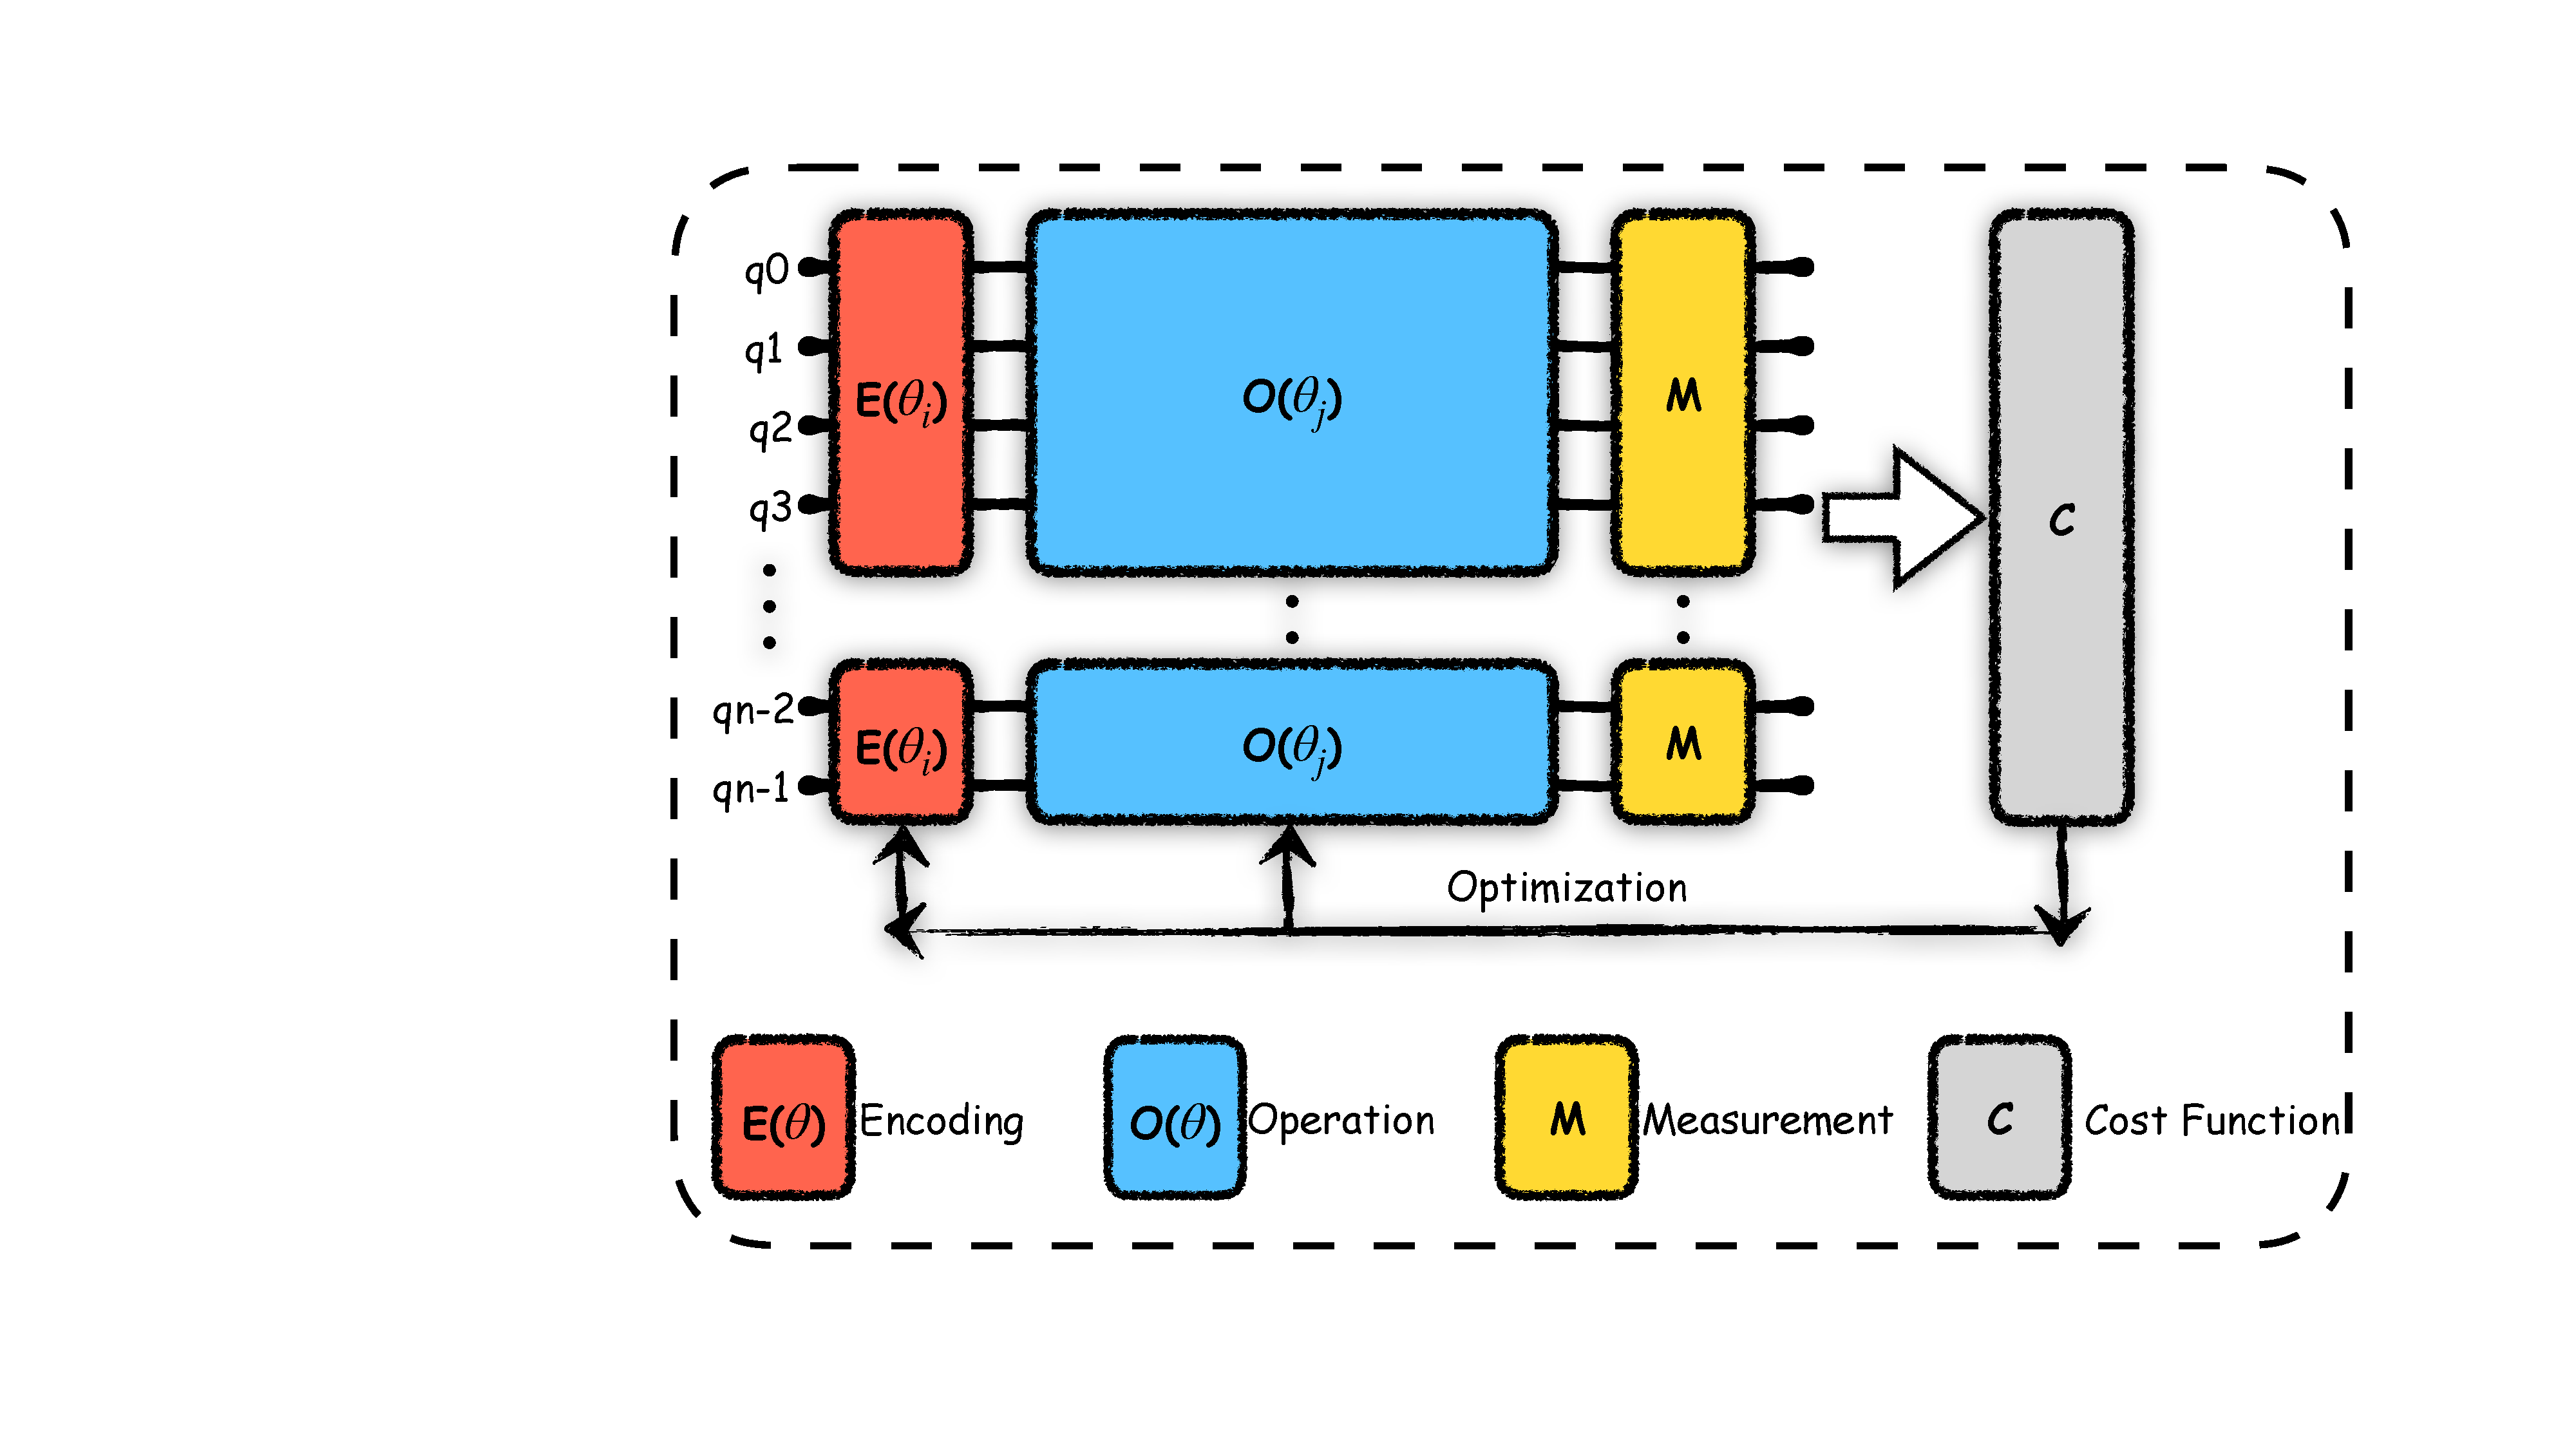
\includegraphics[width=\linewidth,trim=0 0 0 0,clip]{figure/VQC.pdf}
    \end{column}
  \end{columns}
\end{frame}

\begin{frame}{Background-Barren Plateau}
    \begin{columns}[T,totalwidth=\textwidth]
    \begin{column}{0.48\textwidth}
      \begin{KeyBox}[Defination \& Consequence]
        \begin{enumerate}\itemsep4pt
          \item Gradients vanish exponentially with qubit number or circuit depth.
          \item Random init, deep depth, cost function choice.
          \item Training stalls, no effective learning.
          \item Like a flat desert, no slope to follow.
        \end{enumerate}
      \end{KeyBox}
    \end{column}
    \begin{column}{0.5\textwidth}
      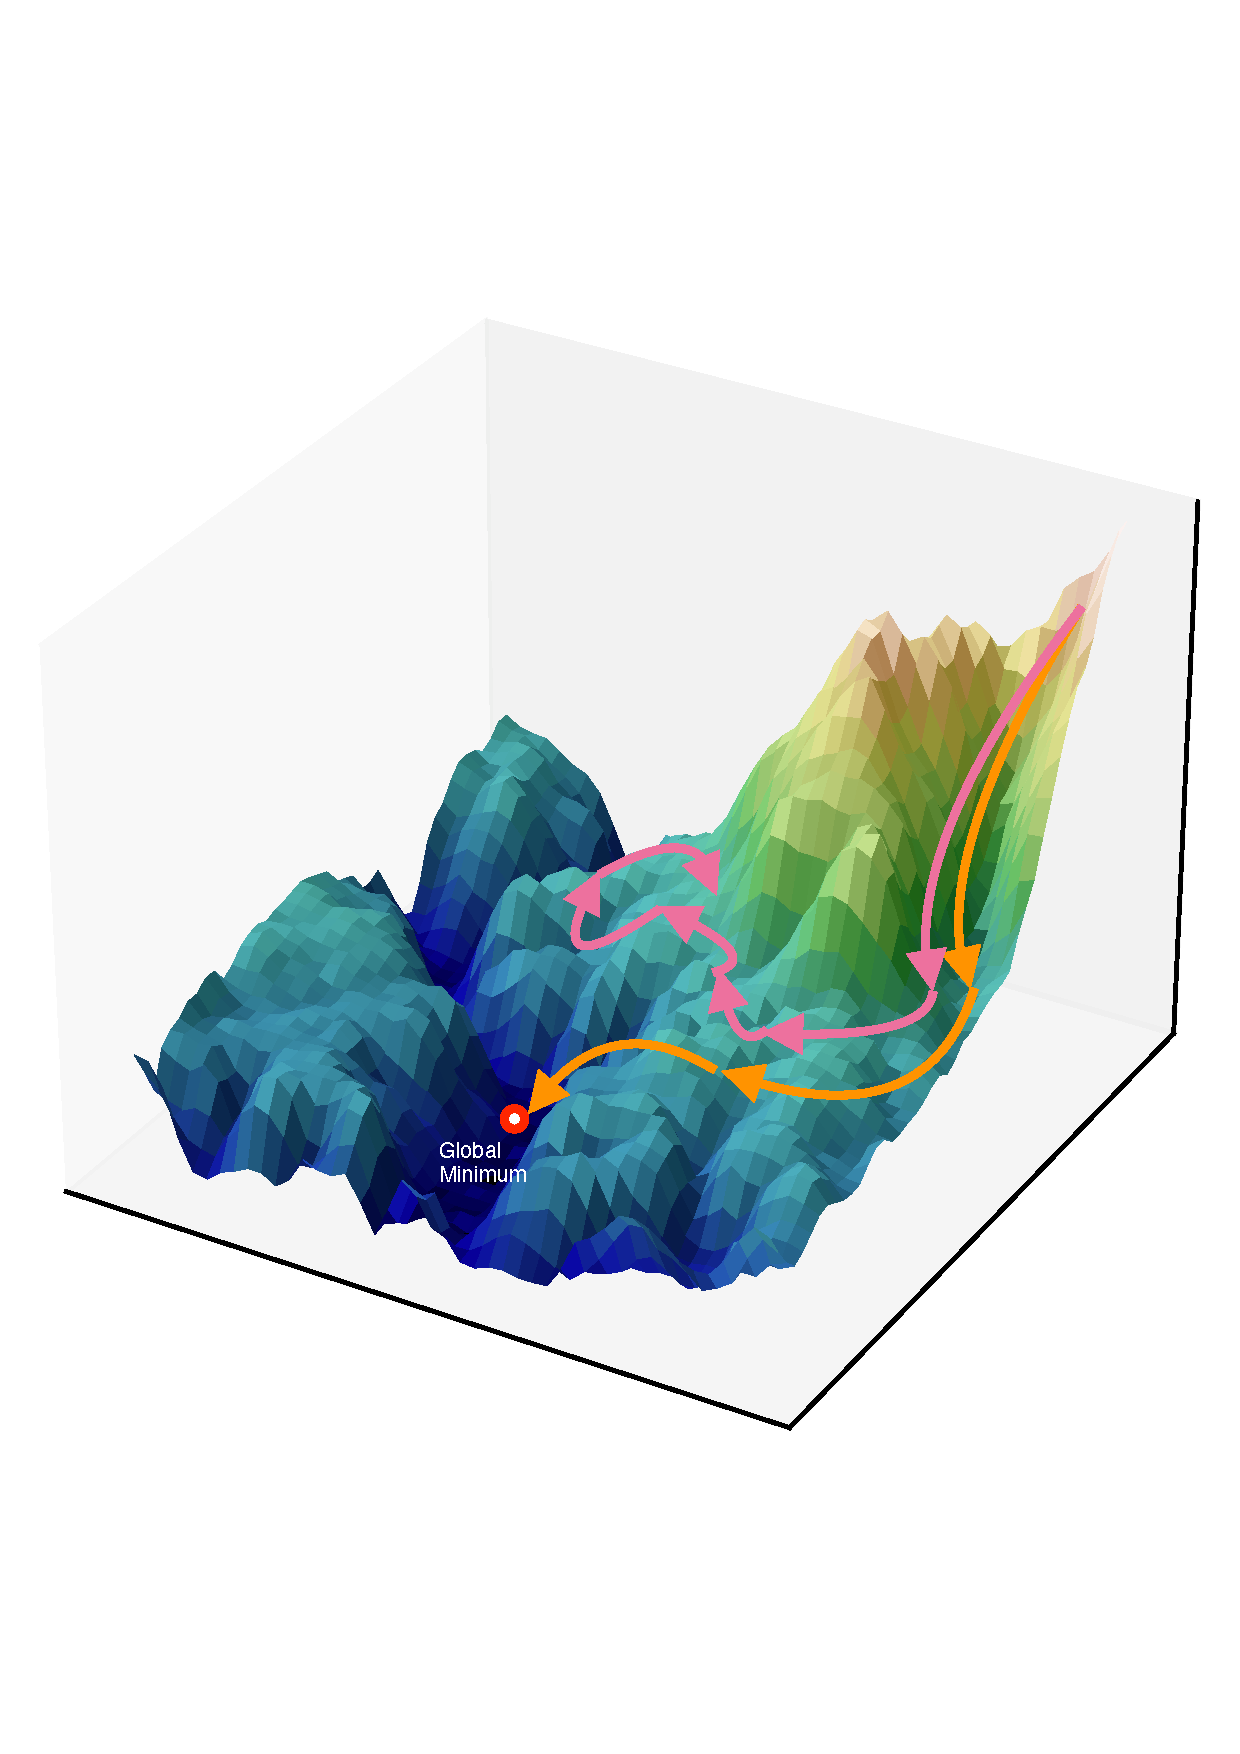
\includegraphics[width=\linewidth,trim=0 0 0 0,clip]{figure/bp.pdf}
    \end{column}
  \end{columns}
\end{frame}

\begin{frame}{Background-Deep Learning Inspired Method}
    \begin{KeyBox}[]
  \begin{itemize}\itemsep4pt
    \item \textbf{Residual Network}: Res-Net introduces 'shortcut connections' to implement residual learning, enabling the training of ultra-deep networks by mitigating the degradation problem.\cite{he2016}.
    \begin{equation*}
      \mathbb{H}(x) = \mathbb{F}(x) + x
    \end{equation*}
    \item \textbf{ResQNets}: ResQNets mitigate the barren plateau problem by partitioning deep architectures into independent PQC nodes and implementing residual connections where the measurement outcomes of preceding nodes are added to the original input for subsequent processing \cite{kashif2024}.
  \end{itemize}
  \end{KeyBox}
  \begin{NoteBox}
  However, intermediate measurements trigger state collapse and decoherence. A critical question remains: Can we implement residual connections without intermediate measurements to preserve quantum coherency until the final output?
  \end{NoteBox}
\end{frame}

\begin{frame}{Method}
    \begin{KeyBox}[Introduce a Messenger Qubit]
  \begin{itemize}\itemsep4pt
    \item Information Collection.
    \item Information Distribution.
  \end{itemize}
  \end{KeyBox}
\begin{figure}[htbp]
    \centering
    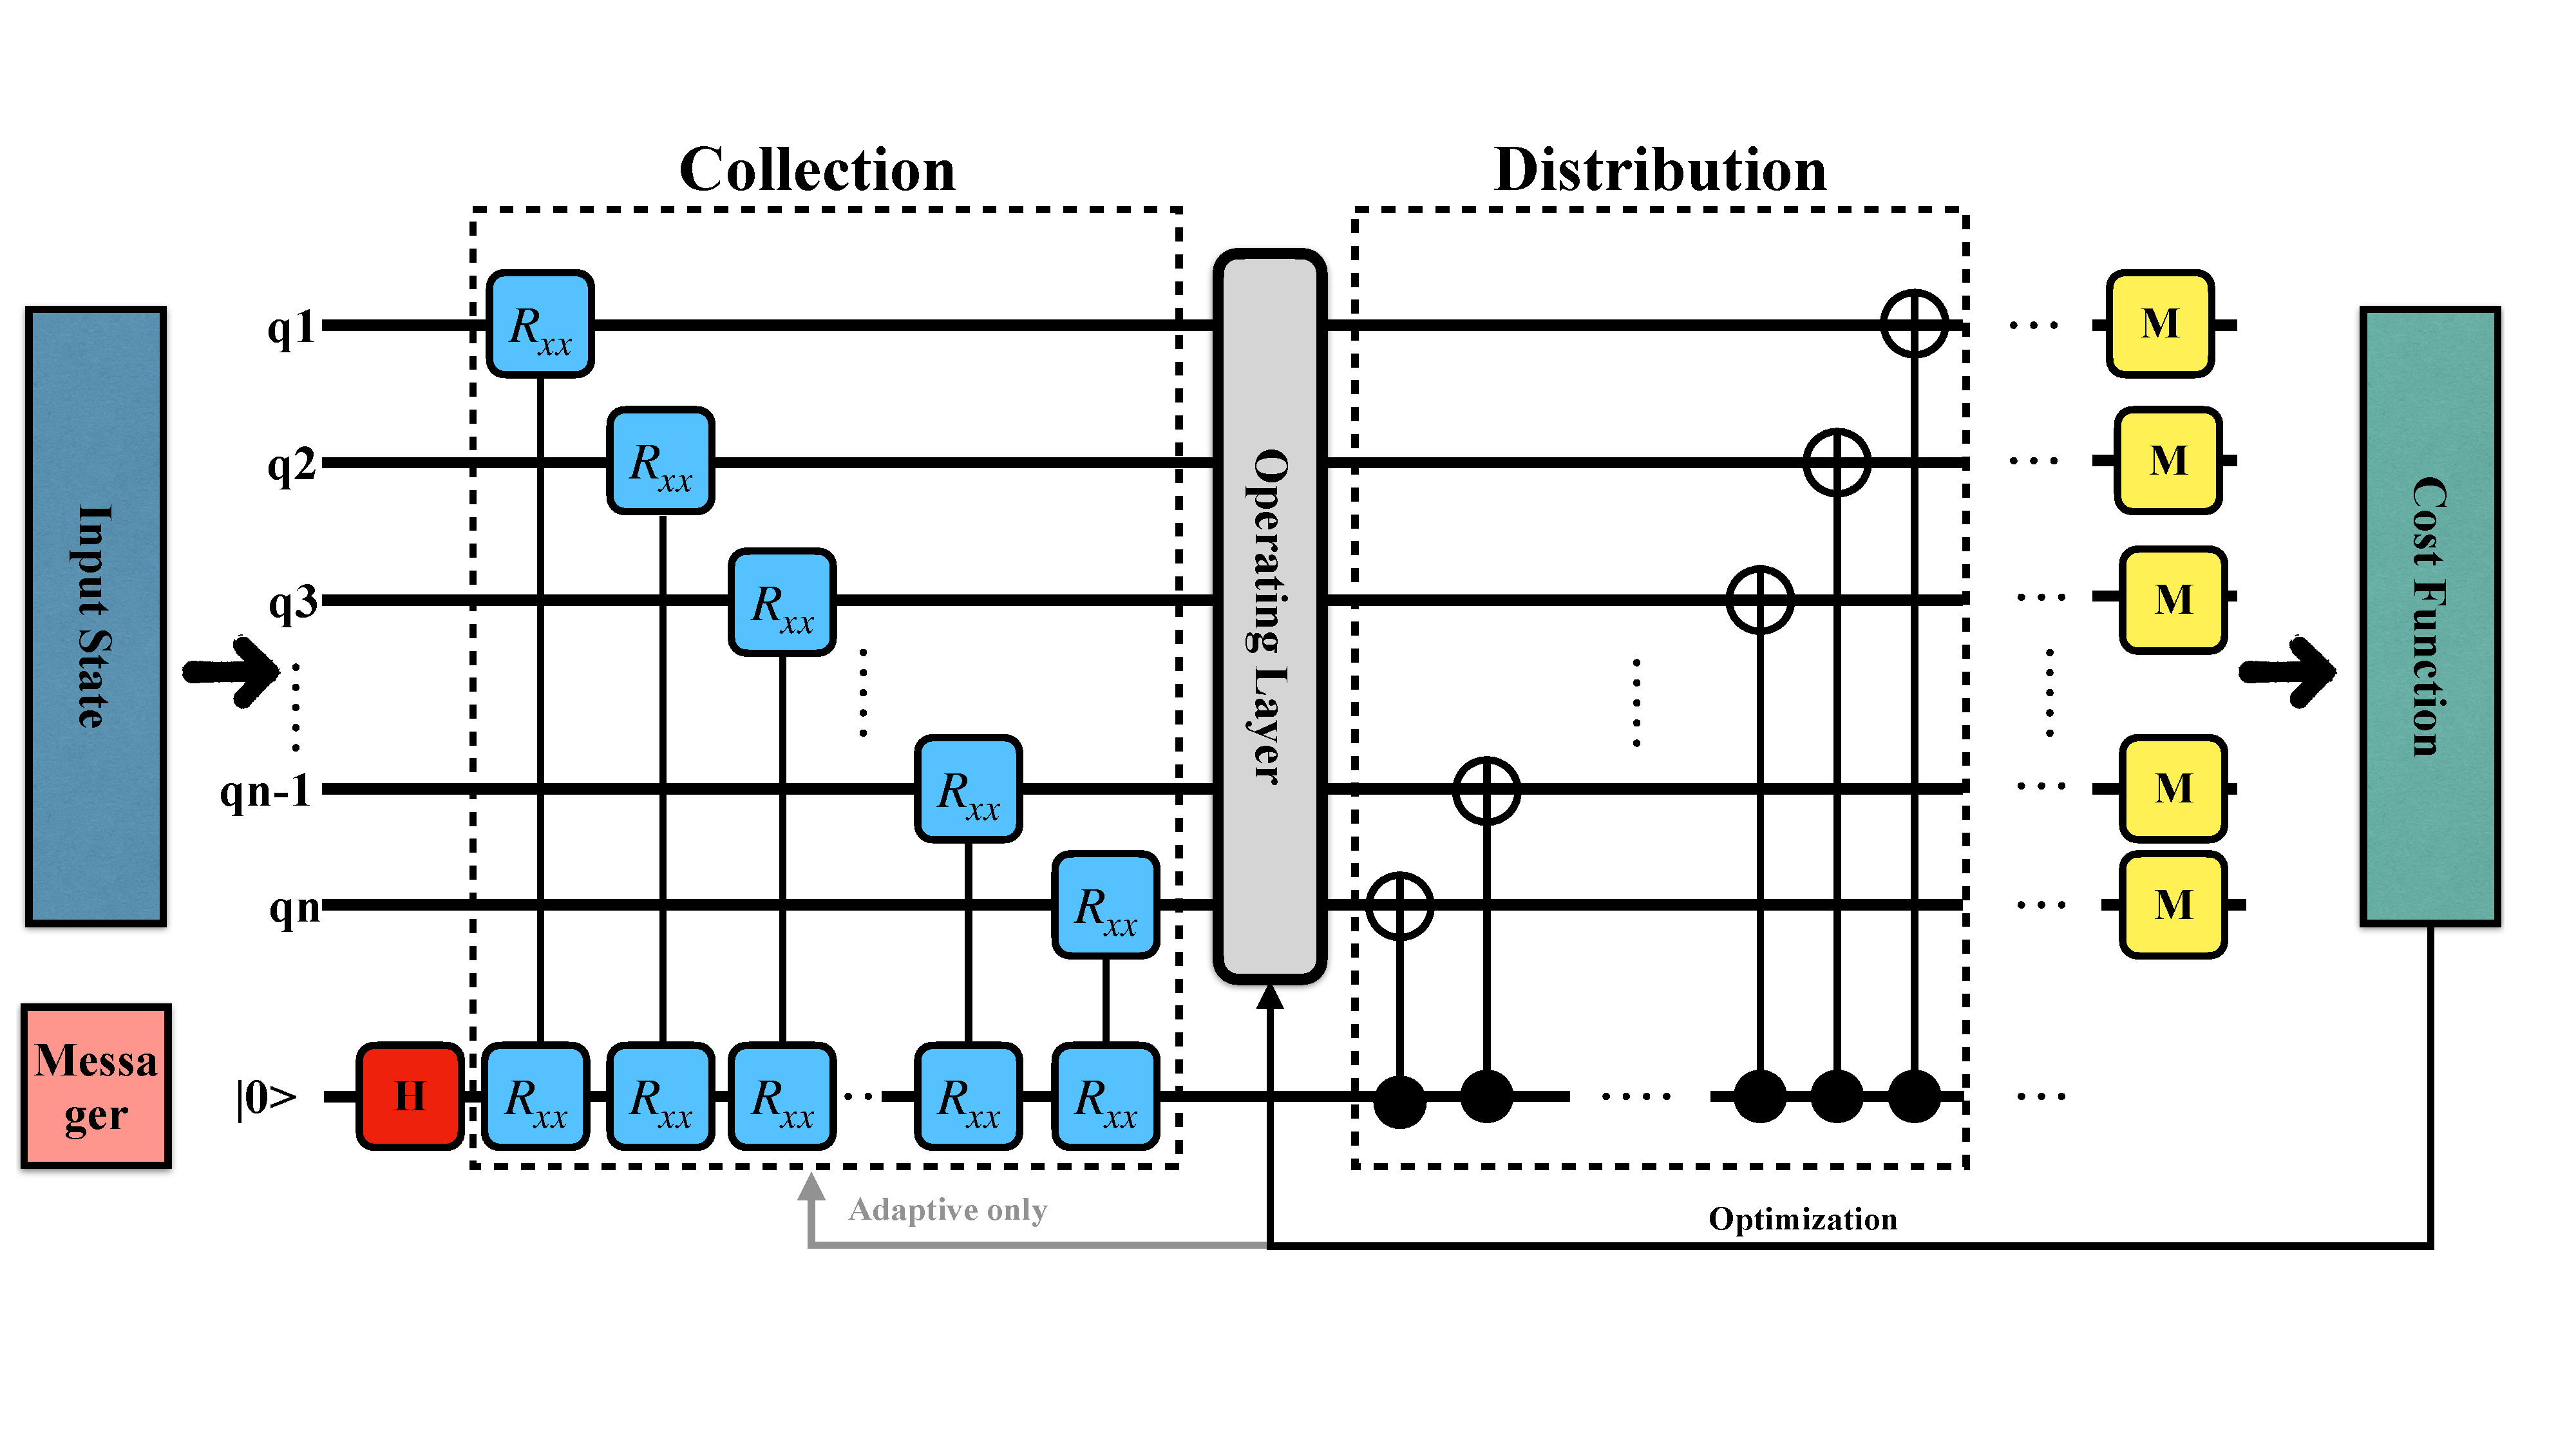
\includegraphics[width=0.6\textwidth]{figure/QLINK.pdf}
    \caption{Messenger Qubit Design}
    \label{fig: messenger_qubit}
\end{figure}
\end{frame}

\begin{frame}{Method}
    \begin{KeyBox}[Introduce a Messenger Qubit]
  \begin{itemize}\itemsep4pt
    \item \textbf{Information Collection}: Employs a Messenger Qubit (initialized at $\ket{0}$) to interact with each Data Qubit via $R_{xx}$ gates.
    \item \textbf{Information Distribution}: Post-operation, the Messenger Qubit re-interacts with Data Qubits via CNOT gates.
  \end{itemize}
  \end{KeyBox}
\end{frame}

\begin{frame}{Method}
    \begin{KeyBox}[Unitary Evolution and Structural Variants]
  \begin{itemize}\itemsep4pt
    \item \textbf{Preservation of Unitarity}
    \begin{itemize}
      \item Unitary Operator: The entire module is represented as $U_{Q-LINK} = U_{dist} U_{opr} U_{coll}$.
      \item Unlike previous works that rely on measurement-based classical feedback, Q-LINK maintains a fully unitary structure, preserving quantum coherence and entanglement throughout the circuit
    \end{itemize}
    \item \textbf{Two Structural Variants}
    \begin{itemize}
      \item Q-LINK (Fixed): Provides a stable, non-trainable way for information flow.
      \item Q-LINK (Adaptive): Offers higher flexibility to capture complex correlations in larger-scale systems.
    \end{itemize}
  \end{itemize}
  \end{KeyBox}
\end{frame}

\begin{frame}{Convergence Speed}
    \begin{columns}[T, onlytextwidth] 
        
        \begin{column}{0.48\textwidth}
            \begin{KeyBox}[Results]
                \begin{enumerate}\itemsep8pt
                    \item \textbf{Baseline (Vanilla)}: requires exponentially more iterations as qubits grow.
                    \item \textbf{Q-LINK (Fixed)}: achieves the fastest convergence across all scales.
                    \item \textbf{Q-LINK (Adaptive)}: slower than Fixed due to the complexity of a richer parameter space.
                \end{enumerate}
            \end{KeyBox}
        \end{column}


        \begin{column}{0.5\textwidth}
            \vspace{0pt} 
            \centering
            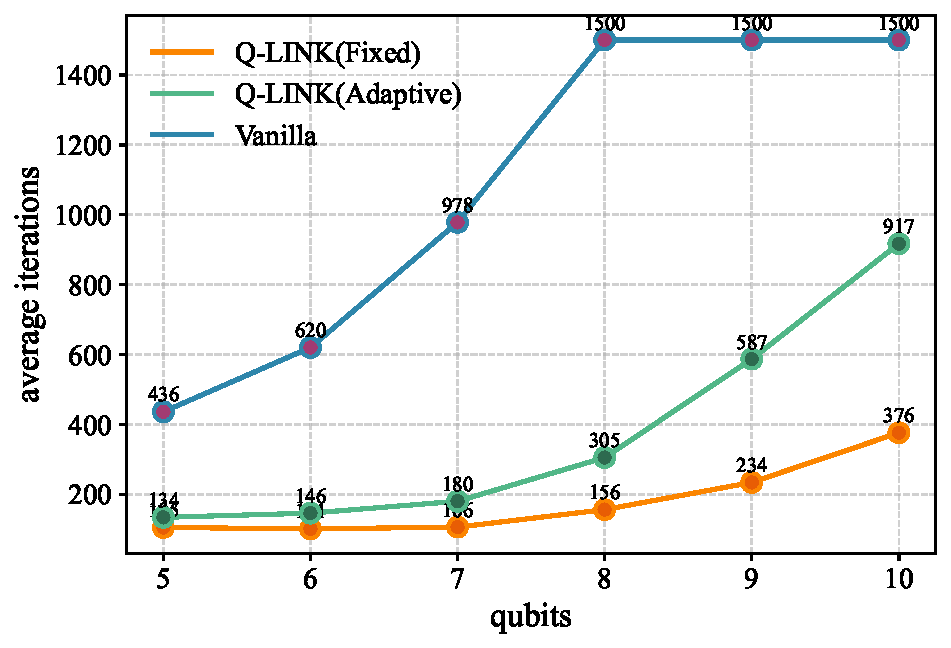
\includegraphics[width=\linewidth, keepaspectratio]{figure/avgiter_vs_qubits.pdf}
            \small\textit{Figure: Iterations to convergence vs. Number of Qubits}
        \end{column}
        
    \end{columns}
\end{frame}

\begin{frame}{Loss Landscape Analysis (8 Qubits)}
    \begin{columns}[t, onlytextwidth]
        \begin{column}{0.32\textwidth}
            \centering
            \small Vanilla\\
            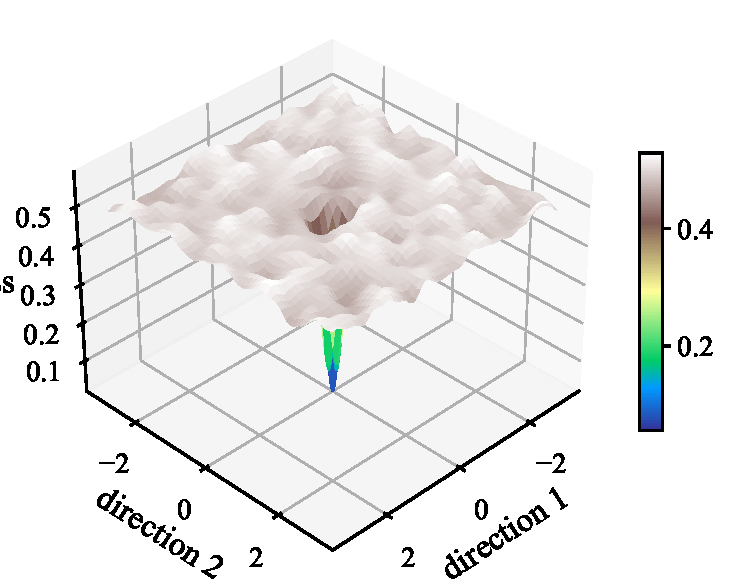
\includegraphics[width=\linewidth]{figure/n8_Vanilla_landscape.pdf}
        \end{column}
        \begin{column}{0.32\textwidth}
            \centering
            \small Q-LINK (Fixed)\\
            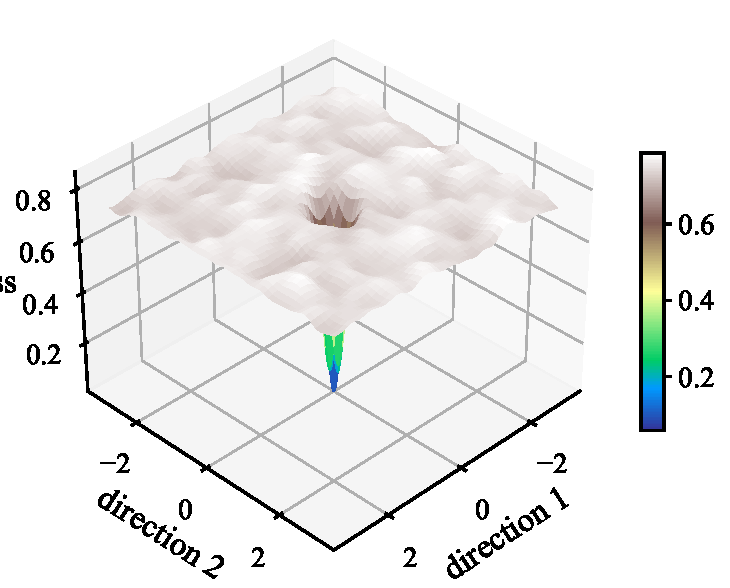
\includegraphics[width=\linewidth]{figure/n8_Q-LINK(Fixed)_landscape.pdf}
        \end{column}
        \begin{column}{0.32\textwidth}
            \centering
            \small Q-LINK (Adaptive)\\
            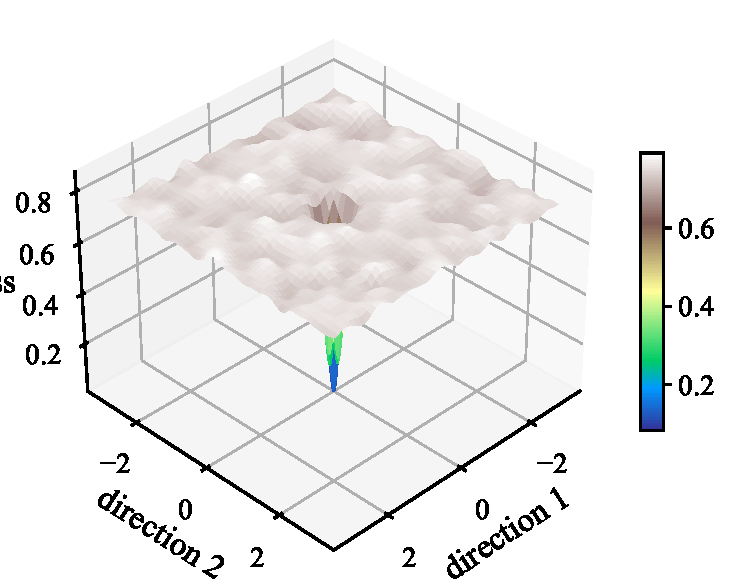
\includegraphics[width=\linewidth]{figure/n8_Q-LINK(Adaptive)_landscape.pdf}
        \end{column}
    \end{columns}

    \begin{KeyBox}[Key Observations]
        \begin{itemize}
            \item \textbf{Local Minima}: Vanilla is riddled with "hill-like" local traps, whereas Q-LINK provides a more clear, obstacle-free path to the optimum.
            \item \textbf{Resilient}: As qubits scale, Q-LINK maintains a smooth and trainable landscape, effectively overcoming the barren plateau problem.
        \end{itemize}
    \end{KeyBox}
\end{frame}

\begin{frame}{Quantitative Analysis: Expressibility \& Gradients}
    \begin{columns}[c, onlytextwidth]
        \begin{column}{0.38\textwidth}
            \begin{KeyBox}[Key Insights]
                \begin{itemize}
                    \item \textbf{High Expressibility}.
                    \item \textbf{Gradient Preservation}: 
                        \begin{itemize}
                            \item \textbf{Vanilla} variance drops to $10^{-7}$ (Barren Plateau).
                            \item \textbf{Q-LINK} variants maintain variance up to \textbf{2 orders of magnitude} higher, ensuring effective training at larger scales.
                        \end{itemize}
                \end{itemize}
            \end{KeyBox}
        \end{column}

        
        \begin{column}{0.6\textwidth}
            \centering
            \tiny 
            \renewcommand{\arraystretch}{1.1} 
            \begin{tabular}{c l c c}
                \toprule
                \textbf{Qubits} & \textbf{Model} & \textbf{Expressibility} & \textbf{Grad. Var.} \\
                \midrule
                \multirow{3}{*}{6} 
                & Q-LINK(Fixed) & $7.55\times 10^{-3}$ & $2.81\times 10^{-5}$ \\
                & Q-LINK(Adaptive) & $3.03\times 10^{-3}$ & $1.25\times 10^{-5}$ \\
                & Vanilla & $3.62\times 10^{-3}$ & $2.74\times 10^{-6}$ \\
                \hline
                \multirow{3}{*}{8} 
                & Q-LINK(Fixed) & $2.00\times 10^{-6}$ & $5.38\times 10^{-6}$ \\
                & Q-LINK(Adaptive) & $2.00\times 10^{-6}$ & $1.60\times 10^{-5}$ \\
                & Vanilla & $8.40\times 10^{-5}$ & $6.02\times 10^{-7}$ \\
                \hline
                \multirow{3}{*}{10} 
                & Q-LINK(Fixed) & $0$ & $9.62\times 10^{-7}$ \\
                & Q-LINK(Adaptive) & $0$ & $7.27\times 10^{-6}$ \\
                & Vanilla & $0$ & $1.18\times 10^{-7}$ \\
                \bottomrule
            \end{tabular}
            \vspace{5pt}
            \\ \textit{*Full data (5-10 qubits) provided in the paper.}
        \end{column}
    \end{columns}
\end{frame}

\begin{frame}{}
  \begin{block}{Summary}
        \begin{itemize}
            \item \textbf{Messenger Mechanism}: Achieves residual learning while \textbf{preserving unitarity} (no state collapse).
            \item \textbf{Barren Plateau Mitigation}: Sustains gradients up to \textbf{100x} larger than Vanilla models.
            \item \textbf{Faster Convergence}: Improves optimization efficiency by \textbf{4-6 times}.
        \end{itemize}
    \end{block}

    \begin{block}{Future Outlook}
        \begin{itemize}
            \item \textbf{Multi-Messenger}: Exploring complex correlations in large-scale QNNs.
            \item \textbf{Real Hardware}: Implementation on NISQ devices to test noise resilience.
            \item \textbf{New Domains}: Applying Q-LINK to VQE and quantum chemistry tasks.
        \end{itemize}
    \end{block}
\end{frame}


\begin{frame}{References}
  \begin{thebibliography}{99}

    \bibitem{he2016}
    K. He, X. Zhang, S. Ren and J. Sun,
    Deep residual learning for image recognition,
    \emph{Proceedings of the IEEE Conference on Computer Vision and Pattern Recognition (CVPR)}, 770-778 (2016).

    \bibitem{kashif2024}
    M. Kashif and S. Al-Kuwari,
    ResQNets: a residual approach for mitigating barren plateaus in quantum neural networks,
    \emph{EPJ Quantum Technology}, 11, 4 (2024).
  \end{thebibliography}
\end{frame}

\begin{frame}{}
  \centering
  {\LARGE \color{UAHBlueDeep} \textbf{Thank you!}}\\[6pt]
  \faIcon{envelope}~\texttt{zhehao.yi@uah.edu} \\[4pt]
  \text{Lab: https://aarc-lab.github.io/} \\
  \begin{center}
    \raisebox{-0.5\height}{
\includegraphics[height=2.5cm]{figure/UAH_Horizontal_2025UPDATE_RGB_01.png}}
    \hspace{1.2cm}
    \raisebox{-0.5\height}{
\includegraphics[height=2.0cm]{figure/LogoWithText.pdf}}
  \end{center}
\end{frame}

\end{document}
